%- block legend
Mário está em sua jornada pelo reino dos cogumelos para salvar a princesa.
Em determinada fase, Mário encontrou uma capa mágica que o permite voar. Mário
então subiu em uma plataforma e pulou dela com a capa. Você percebeu que:
\begin{itemize}
    \item Mário pulou da plataforma a uma altura de $h_0$ metros;
    \item a trajetória do pulo teve o formato de uma parábola, com a concavidade para cima;
    \item a $x_1$ metros de distância (horizontal) da plataforma, Mário estava a uma altura de $h_1$ m;
    \item a $x_2$ metros de distância (horizontal) da plataforma, Mário estava a uma altura de $h_2$ m;
    \item Mário não tocou o chão em nenhum momento.
\end{itemize}

\begin{center}
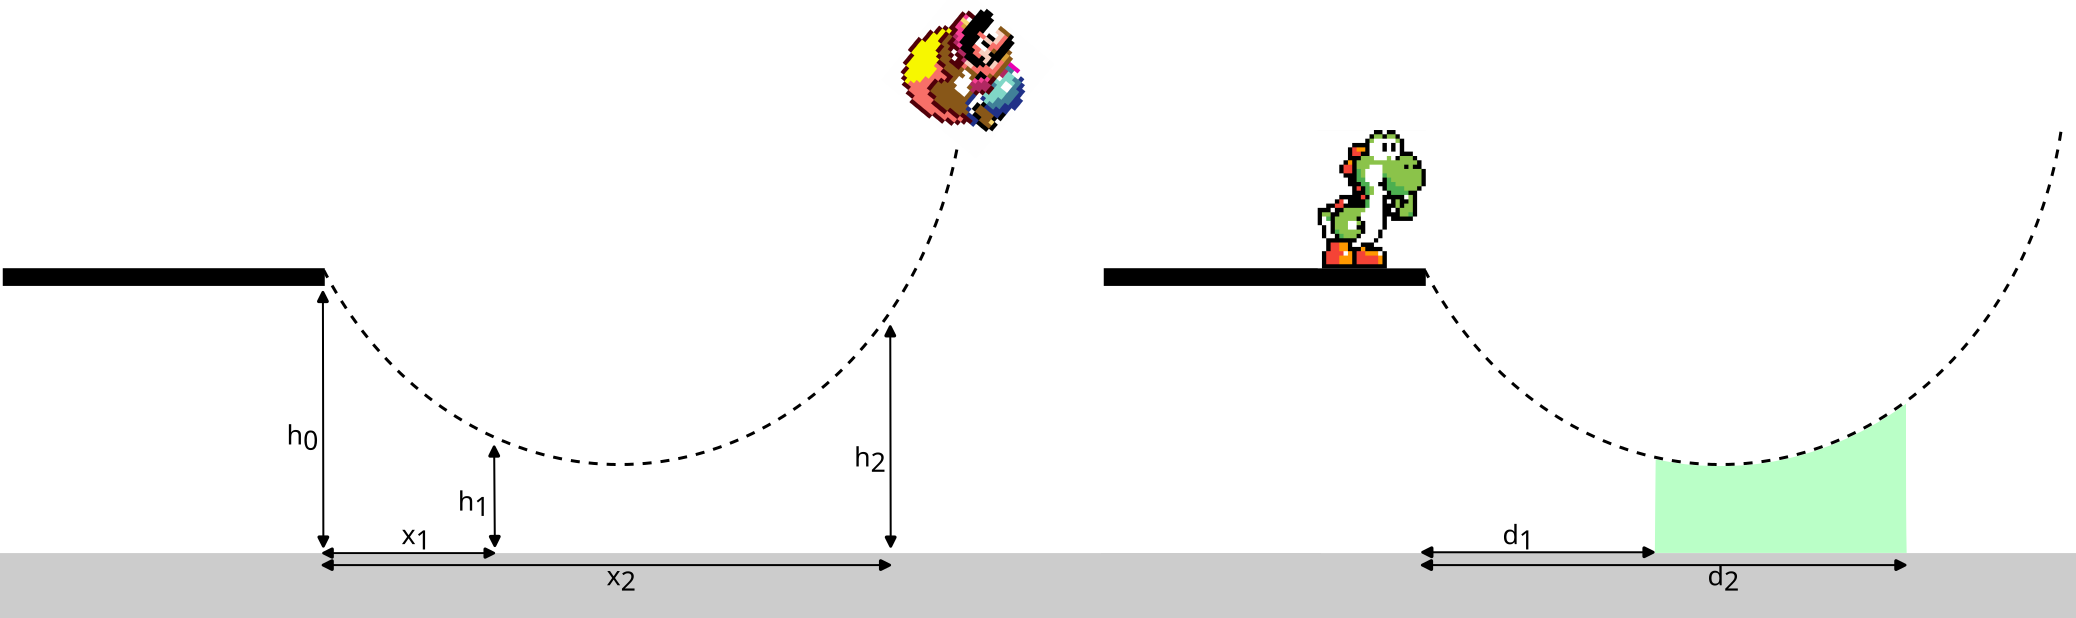
\includegraphics[scale=0.3]{jornada.png}
\end{center}

Yoshi, o dinossauro ajudante do Mário, está com medo de que Mário perca uma vida
e, na próxima tentativa, faça o pulo em com ele junto (podendo,
tragicamente, deixar Yoshi para trás durante o pulo!). Yoshi precisa calcular
suas chances de sobrevivência; para isso, dadas duas distâncias
$d_1$ e $d_2$ metros (horizontais) da plataforma, ajude Yoshi a calcular a área
abaixo da trajetória que Mário fez entre $d_1$ e $d_2$.

%- endblock

%- block input
A primeira linha contém um inteiro $T$, o número de casos de teste
$(\VAR{T.min} \leq T \leq \VAR{T.max | sci})$.\\
Cada caso de teste é dado um uma linha com sete inteiros
$h_0$, $x_1$, $y_1$, $x_2$, $y_2$, $d_1$ e $d_2$\\
$(\VAR{N.min} \leq h_0, x_1, y_1, x_2, y_2, d_1, d_2 \leq \VAR{N.max},
x_1 \neq x_2, d_1 < d_2)$.
É garantido que a entrada é tal que a concavidade da trajetória é
para cima e que ela não toca o chão.
%- endblock

%- block output
Para cada caso teste, imprima a área pedida, em metros quadrados.\\
A resposta será considerada correta se seu erro absoluto (diferença entre sua
        resposta e a resposta exata) for menor ou igual a $10^{-6}$.
%- endblock

%- block editorial
Primeiramente, vamos descobrir a equação da parábola que representa a
trajetória. Ela é dada uma função de segundo grau, na forma $f(x) = Ax^2 + Bx + C$.
Precisamos descobrir os valores dos coeficientes $A$, $B$ e $C$.

Tem-se que $f(0) = h_0$; logo, $C=h_0$. Para os
outros coeficientes, temos o seguinte sistema de equações lineares:

$\begin{cases}
A(x_1)^2 + Bx_1 = h_1 - C\\
A(x_2)^2 + Bx_2 = h_2 - C
\end{cases}$

ou, na forma matricial,

$\begin{bmatrix}
(x_1)^2 & x_1 \\
(x_2)^2 & x_2 \\
\end{bmatrix}
.
\begin{bmatrix}
A \\
B \\
\end{bmatrix} =
\begin{bmatrix}
h_1 - C\\
h_2 - C\\
\end{bmatrix}
$
.

Há diversos algoritmos para se resolver sistemas de equações lineares. Para o
caso geral, veja \url{https://cp-algorithms.com/linear\_algebra/linear-system-gauss.html}
para um algoritmo cúbico.
Mas, por se tratar de um sistema pequeno $2 \times 2$, você também pode resolvê-lo por
substituição direta em $O(1)$.

Com a função $f(x) = Ax^2 + Bx + C$ definida, podemos calcular a área utilizando
Cálculo Integral. A área é dada por

$\displaystyle\int_{d_1}^{d_2} Ax^2 + Bx + C\,dx$
$\displaystyle = \frac{Ax^3}{3} + \frac{Bx^2}{2} + Cx\, \Big|_{d_1}^{d_2}$
$\displaystyle = \frac{A(d_2)^3}{3} + \frac{B(d_2)^2}{2} + Cd_2
- \frac{A(d_1)^3}{3} - \frac{B(d_1)^2}{2} - Cd_1$.

Complexidade: $O(1)$ por caso de teste.

%- endblock
